\documentclass[11pt,spanish]{article}
\usepackage[utf8]{inputenc}
\usepackage{babel}
\usepackage{fullpage}
\usepackage{listings}
\usepackage{mathpazo}
\usepackage{enumitem}
\usepackage{courier}
\usepackage{textcomp}
\usepackage{amsmath}
\usepackage{tikz}
\usepackage{fancyhdr}

\hyphenation{usua-rio usua-rios}

\newcommand{\titulo}{Certamen 2, sábado 14 de mayo de 2011}

\pagestyle{fancy}
\lhead{%
  {\Large\bfseries Programación---\titulo} \\
  Nombre: \nombre\hfill
  Rol:    \rol
  \vspace{2ex}
}
\chead{}\rhead{}\lfoot{}\cfoot{}\rfoot{}
\renewcommand{\headrulewidth}{0pt}
\addtolength{\headheight}{7ex}
\headsep=4ex


\newcommand{\onelinerule}{\rule[2.3ex]{0pt}{0pt}}
\newcommand{\twolinerule}{\rule[6.2ex]{0pt}{0pt}}
\newcommand{\respuesta}{\framebox[\textwidth]{\twolinerule}}
\newcommand{\nombre}{%
  \begin{tikzpicture}[xscale=.4,yscale=.7]
    \draw (0, 0) rectangle (22, 1);
  \end{tikzpicture}%
}
%\newcommand{\rol}   {\framebox[0.3\textwidth]{\onelinerule}}
\newcommand{\rol}{%
  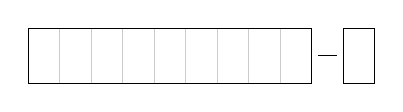
\begin{tikzpicture}[xscale=.4,yscale=.7]
    \draw[gray!40] ( 0, 0) grid      ( 9, 1);
    \draw          ( 0, 0) rectangle ( 9, 1);
    \draw          (10, 0) rectangle (11, 1);
    \draw (9 + .2, .5) -- (10 - .2, .5);
  \end{tikzpicture}%
}
\newcommand{\li}{\lstinline}
\newcommand{\pond}[1]{[{\small\textbf{#1\%}}]}

\lstdefinelanguage{py}{%
  classoffset=0,%
    morekeywords={%
      False,class,finally,is,return,None,continue,for,lambda,try,%
      True,def,from,nonlocal,while,and,del,global,not,with,print,%
      as,elif,if,or,yield,assert,else,import,pass,break,except,in,raise},%
    keywordstyle=\color{black!80}\bfseries,%
  classoffset=1,
    morekeywords={int,float,str,abs,len,raw_input,exit,range,min,max,%
      set,dict,tuple,list,bool,complex,round,sum,all,any,zip,map,filter,%
      sorted,reversed,dir,file,frozenset,open,%
      array,zeros,ones,arange,linspace,eye,diag,dot},
    keywordstyle=\color{black!50}\bfseries,%
  classoffset=0,%
  sensitive=true,%
  morecomment=[l]\#,%
  morestring=[b]',%
  morestring=[b]",%
  stringstyle=\em,%
}

\lstdefinelanguage{testcase}{%
  moredelim=[is][\bfseries]{`}{`},%
  backgroundcolor=\color{gray!20},%
}

\lstdefinelanguage{file}{%
  frame=single,%
  backgroundcolor=\color{white},%
}

\lstset{language=py}
\lstset{basicstyle=\ttfamily}
\lstset{columns=fixed}
\lstset{upquote=true}
\lstset{showstringspaces=false}
\lstset{rangeprefix=\#\ }
\lstset{includerangemarker=false}

\newlist{certamen}{enumerate}{1}
\setlist[certamen]{%
  label=\arabic*.,
  font=\LARGE\bfseries,%
  labelindent=-.5in,%
  leftmargin=0pt,%
  labelsep=1em%
}



\begin{document}
  \begin{enumerate}[font=\Large\bfseries]
    \item
      \pond{25}
      En el idioma de la tribu de los Stringones,
la mayoría de las palabras tienen muchas letras
que se repiten de manera consecutiva.

El sabio de la tribu ideó un sistema
para escribir las palabras de manera abreviada:
cada letra aparece antecedida de un número,
indicando cuántas veces está repetida.
Por ejemplo, la palabra \li!pppprrrrrogggrraaa!
se abrevia \li!4p5r1o3g2r3a!.

Desarrolle un programa
que reciba como entrada una palabra abreviada,
y entregue como salida la palabra original.
Suponga que ninguna letra
aparece más de nueve veces seguidas.


      \newpage
    \item
      \pond{25}
      En el idioma de la tribu de los Stringones,
la mayoría de las palabras tienen muchas letras
que se repiten de manera consecutiva.

El sabio de la tribu ideó un sistema
para escribir las palabras de manera abreviada:
cada letra aparece antecedida de un número,
indicando cuántas veces está repetida.
Por ejemplo, la palabra \li!pppprrrrrogggrraaa!
se abrevia \li!4p5r1o3g2r3a!.

Desarrolle un programa
que reciba como entrada una palabra abreviada,
y entregue como salida la palabra original.
Suponga que ninguna letra
aparece más de nueve veces seguidas.


      \newpage
    \item
      \pond{25}
      La banda de rock Strip'n Split
ha concluído su gira mundial.
La información de cada uno de sus conciertos
está almacenada en una lista
en orden cronológico.

\begin{minipage}[t]{.45\textwidth}
  Cada elemento de la lista
  es un diccionario con tres llaves:
  \li!'ciudad'!, \li!'publico'! y \li!'canciones'!.
  El valor asociado a \li!'publico'!
  es la cantidad de personas que asistió al concierto,
  y el asociado a \li!'canciones'!
  es la lista de las canciones que fueron tocadas
  en ese concierto.

  \begin{enumerate}
    \item
      Escriba una función llamada
      \li!cuantos_escucharon(c)!,
      que retorne la cantidad de personas
      que escucharon la canción \li!c!.
    \item
      Escriba una función llamada
      \li!mismo_concierto(c1, c2)!,
      que retorne \li!True! o \li!False!
      para indicar si las canciones \li!c1! y \li!c2!
      fueron tocadas alguna vez en el mismo concierto.
  \end{enumerate}
\end{minipage}
\hspace{2em}
\begin{minipage}[t]{.55\textwidth}
  \small
  \lstinputlisting[linerange=CONCIERTOS-FIN\ CONCIERTOS]
     {strip-n-split/pauta3-4.py}
\end{minipage}


      \newpage
    \item
      \pond{25}
      (Este ejercicio es una continuación del anterior).

El diccionario \li!ciudades!
asocia a cada país
una lista de las ciudades de ese país
en las que tocó Strip'n Split:
\lstinputlisting[linerange=CIUDADES-FIN\ CIUDADES]
   {strip-n-split/pauta3-4.py}

\begin{enumerate}
  \item Escriba la función \li!canciones_pais(p)!,
    que retorne el conjunto de las canciones
    que fueron tocadas en el país \li!p!.
  \item Escriba la función \li!contar_exitos(n)!,
    que retorne la cantidad de veces en que
    hubo dos conciertos consecutivos
    en el mismo país
    que tuvieron más de \li!n! espectadores.
\end{enumerate}


  \end{enumerate}
\end{document}

